\documentclass[11pt,a4paper,twocolumn]{article}

% --- Standard Overleaf-safe ACL/EMNLP-like layout ---
% To submit to ARR / ACL / EMNLP, replace geometry + authblk below with:
%   \usepackage[review]{acl}
\usepackage[margin=2.0cm,columnsep=0.65cm]{geometry}
\usepackage[T1]{fontenc}
\usepackage[utf8]{inputenc}
\usepackage{times}
\usepackage{latexsym}
\usepackage{amsmath,amssymb}
\usepackage{booktabs}
\usepackage{multirow}
\usepackage{graphicx}
\usepackage{microtype}
\usepackage{natbib}
\usepackage{xcolor}
\usepackage{hyperref}

\hypersetup{
  colorlinks=true,
  linkcolor=blue!60!black,
  citecolor=blue!60!black,
  urlcolor=blue!60!black
}

\graphicspath{{../results/figures/}{figures/}}

\title{\textbf{Cross-Lingual Calibration Bias in Low-Rank KV-Cache Compression:\\Attention Sinks, QK-Norm Amplification, and Low-Resource Recovery}}

\author{
  \textbf{Maria Contreras}\\
  Disentangle Lab\\
  \texttt{https://github.com/Disentangle-Lab/kv-cache-low-resources}
}
\date{}

\begin{document}
\maketitle

% ============================================================================
\begin{abstract}
Low-rank Key--Value (KV) cache compression reduces LLM inference memory by projecting cached states onto top singular subspaces estimated from a calibration corpus---almost always English. We conduct a systematic empirical study of cross-lingual calibration bias across English (\texttt{en}), Spanish (\texttt{es}), Finnish (\texttt{fi}), and Ayacucho Quechua (\texttt{qu}) on two architectures with identical KV geometry ($28$ layers, $8$ KV heads, $d=128$): \textbf{Qwen3-1.7B} (with per-head QK-RMSNorm, \texttt{k\_norm}) and \textbf{Llama-3.2-3B} (without \texttt{k\_norm}).
Our experiments establish four findings.
First, \textbf{Value (\texttt{V}) states carry severe cross-lingual calibration bias across network depth, whereas Key (\texttt{K}) states are nearly language-agnostic once the position-0 attention sink is protected}: on strictly parallel FLORES-200 translations ($r=0.25d$), English-only calibration of late-layer \texttt{V} penalizes Quechua by $+0.601$ nats/token ($+75.1\%$ PPL) on Qwen3 and $+0.524$ ($+72.1\%$) on Llama-3.2, and Finnish by $+0.601$ ($+90.3\%$) on Llama-3.2, while \texttt{K} stays within $|\Delta\text{NLL}|\le 0.032$ across all depth quartiles.
Second, \textbf{standard full-sequence SVD fails to preserve the position-0 attention sink in \texttt{K}}, causing moderate degradation on Llama-3.2 ($+5.1$--$10.6\%$) and a catastrophic $+153$--$328\%$ explosion on Qwen3 due to \texttt{k\_norm} amplifying angular distortion ($\cos=0.689$ at position~0); protecting just \emph{one} sink token eliminates this failure ($-0.37\%$ to $+2.0\%$ PPL).
Third, \textbf{leave-one-out multilingual calibration (\texttt{multi\_loo}) fails to rescue unseen low-resource languages, but mixing just $\sim$5k tokens of the target language ($w=0.10$) into a layer-wide shared (\texttt{joint}) projector closes 97--100\% of the parallel FLORES-200 gap}---even cross-domain from Wikipedia to news---and enables viable $4\times$ full-model \texttt{K+V} compression across layers 3--27.
Fourth, on downstream tasks (\textbf{SIB-200} classification and \textbf{FLORES-200} autoregressive translation with real \texttt{use\_cache=True} decoding), English-calibrated $4\times$ compression triggers literal \textbf{language-collapse into English} during \texttt{qu}$\rightarrow$\texttt{es} generation (chrF++ $27.5\rightarrow 13.3/14.0$), whereas our 5k-token multilingual mixture recovers $22.9$--$24.1$ chrF++ and outperforms \emph{every} monolingual basis on bilingual prompts.
\end{abstract}

% ============================================================================
\section{Introduction}
Serving large language models (LLMs) on consumer GPUs or edge hardware is frequently bottlenecked by the Key--Value (KV) cache, whose memory footprint grows linearly with sequence length and batch size. Data-dependent low-rank projection methods---such as Palu \citep{chang2025palu} and Eigen Attention \citep{saxena2024eigen}---compress cached keys and values by projecting them onto the top-$r$ singular subspace estimated from a small calibration set. In practice, calibration is almost universally performed on English text (e.g., WikiText-2 or C4).

Yet compute-constrained regions that depend most heavily on aggressive inference compression are disproportionately home to speakers of morphologically rich and low-resource languages---a dynamic \citet{marchisio2024quantization} term the \emph{low-resource double bind}. While prior work has documented disparate multilingual degradation under weight quantization and pruning, it remains unknown whether low-rank KV-cache subspaces transfer across typologically distant languages, whether Keys and Values behave symmetrically, and how much target-language calibration data is required to close any gap.

We answer these questions through a seven-stage empirical investigation covering four languages spanning high-resource Indo-European (\texttt{en}, \texttt{es}), agglutinative Finno-Ugric (\texttt{fi}), and low-resource polysynthetic Andean (\texttt{qu}, Ayacucho Quechua), replicated across \textbf{Qwen3-1.7B} \citep{yang2025qwen3} and \textbf{Llama-3.2-3B} \citep{grattafiori2024llama3}. Both models share an identical KV-cache tensor shape ($28$ layers, $8$ grouped-query KV heads, $d=128$, $D_{\text{KV}}=1024$), allowing a clean 1-to-1 architectural contrast between QK-RMSNorm attention (\texttt{Qwen3}) and standard attention (\texttt{Llama-3.2}).

\paragraph{Contributions.}
\begin{enumerate}
  \item \textbf{K/V Cross-Lingual Asymmetry:} Using held-out article splits, parallel FLORES-200 corpora, and paired bootstrap confidence intervals, we show that cross-lingual calibration bias resides almost exclusively in \texttt{V} across every depth quartile, while \texttt{K} is nearly language-agnostic once position~0 is protected.
  \item \textbf{Position-0 Sink Fragility \& QK-Norm Amplification:} We show that even standard unweighted full-sequence SVD (\texttt{SKIP\_FIRST\_TOKENS=0}) breaks the position-0 attention sink in \texttt{K}, and isolate how per-head \texttt{k\_norm} amplifies this into a $+153$--$328\%$ PPL catastrophe on Qwen3 versus $+5$--$11\%$ on Llama-3.2. Protecting a single token (\texttt{pos 0}) resolves both.
  \item \textbf{Practical 5k-Token Recovery for Full-Model $4\times$ Compression:} We show that sharing a single layer-wide KV projector across heads (\texttt{joint}) cuts cross-lingual NLL loss by up to $76\%$ at equal rank budget, and that adding just $\sim$5k target-language tokens ($w=0.10$) to a multilingual Gram mixture eliminates $97$--$100\%$ of the FLORES-200 gap and rescues $4\times$ full-model \texttt{K+V} compression (layers 3--27).
  \item \textbf{Downstream Language-Collapse Validation:} Under real autoregressive \texttt{use\_cache=True} decoding on FLORES-200 translation and SIB-200 classification, English-calibrated $4\times$ compression induces literal language-collapse into English during \texttt{qu}$\rightarrow$\texttt{es} generation, whereas the 5k-token multilingual basis outperforms \emph{all} monolingual bases---including target-matched calibration---on bilingual prompts.
\end{enumerate}

% ============================================================================
\section{Related Work}
\paragraph{Low-Rank KV-Cache Compression.}
Palu \citep{chang2025palu} compresses KV-cache linear projections via low-rank matrix decomposition with grouped head sharing and activation-aware weighting, while Eigen Attention \citep{saxena2024eigen} performs attention directly in low-rank eigen-subspaces of keys and values. \citet{chen2026kvcore} introduce KV-CoRE to benchmark data-dependent low-rank compressibility via normalized effective rank (NER). None of these studies evaluate cross-lingual subspace transfer or low-resource calibration bias.

\paragraph{Attention Sinks and Massive Activations.}
\citet{xiao2024streamingllm} discovered that retaining initial ``attention sink'' tokens stabilizes streaming KV-cache eviction, and \citet{sun2024massive} linked sinks to massive activations emerging in early layers. Our work extends this line to \emph{low-rank projection}: we demonstrate that standard unweighted SVD fails to preserve position~0 because its pre-norm energy share is tiny ($\sim 0.02\%$), and reveal a severe interaction with QK-RMSNorm (\texttt{k\_norm}).

\paragraph{Multilingual Disparity Under Compression.}
\citet{marchisio2024quantization} showed that post-training weight quantization disproportionately degrades non-English and low-resource languages, often masked by coarse automatic metrics. We extend this inquiry to \emph{KV-cache projection}, showing that calibration language---not merely compression ratio---drives massive performance disparities and forced language switching during decoding.

% ============================================================================
\section{Methodology}

\paragraph{Models and Architecture Contrast.}
We evaluate \texttt{Qwen/Qwen3-1.7B} ($28$ layers, $16$ query heads, $8$ KV heads, $d=128$, per-head \texttt{k\_norm}/\texttt{q\_norm}) and \texttt{unsloth/Llama-3.2-3B} ($28$ layers, $24$ query heads, $8$ KV heads, $d=128$, no \texttt{k\_norm}, unquantized weights). Both have identical KV width $D_{\text{KV}}=N_{\text{KV}}\cdot d = 1024$ and identical depth quartiles: \texttt{early} (0--6), \texttt{mid1} (7--13), \texttt{mid2} (14--20), and \texttt{late} (21--27).

\paragraph{Languages, Splits, and Parallel Controls.}
We study English (\texttt{en}), Spanish (\texttt{es}), Finnish (\texttt{fi}), and Ayacucho Quechua (\texttt{qu}).
\begin{itemize}
  \item \textbf{Wikipedia (held-out splits):} From the \texttt{20231101} snapshot, articles ($\ge 500$ chars, truncated to $2048$ tokens for topical diversity) are deterministically partitioned by \texttt{CRC32(article\_id) \% 2} into disjoint \texttt{calib} ($150\text{k}$ tokens; $292\times 512$ windows) and \texttt{eval} ($60\text{k}$ tokens; $117\times 512$ windows) sets. Even matched-language evaluation is strictly out-of-sample, providing a direct noise floor.
  \item \textbf{FLORES-200 (parallel control):} To eliminate Wikipedia topic/length confounders (\texttt{qu} required $964$ short articles vs.\ $477$--$551$ for \texttt{en/es/fi}), we evaluate on exact parallel translations from FLORES-200 \citep{nllb2022flores} (\texttt{eng\_Latn}, \texttt{spa\_Latn}, \texttt{fin\_Latn}, \texttt{quy\_Latn}): $997$ \texttt{dev} sentences (equalized to $53$/$52$ windows $\approx 27\text{k}$ tokens per language for calibration) and $1{,}012$ \texttt{devtest} sentences for evaluation. Tokenizer fertility on identical sentences is $26.8$/$26.4$ (\texttt{en}), $40.8$/$40.6$ (\texttt{es}), $52.9$/$52.3$ (\texttt{fi}), and $55.2$/$54.4$ (\texttt{qu}) tokens/sentence for Qwen3 / Llama-3.2.
  \item \textbf{Downstream benchmarks (zero-leakage):} Calibrating exclusively on Wikipedia, we evaluate 7-shot \textbf{SIB-200} 7-class topic classification ($204$ parallel test items/lang; \citealp{adelani2024sib200}) and 5-shot \textbf{FLORES-200} autoregressive machine translation ($N=80$ parallel sentences across \texttt{qu}$\rightarrow$\texttt{es}, \texttt{es}$\rightarrow$\texttt{qu}, \texttt{fi}$\rightarrow$\texttt{en}, \texttt{es}$\rightarrow$\texttt{en}; scored by corpus/sentence chrF++, \citealp{popovic2017chrf}).
\end{itemize}

\paragraph{Gram SVD Projectors and Calibration Sources.}
For each layer $\ell$ and state kind $X \in \{K, V\}$, we accumulate the per-token normalized uncentered second-moment (Gram) matrix $G_\ell = \frac{1}{N} \sum_{t} x_t x_t^\top \in \mathbb{R}^{D_{\text{KV}} \times D_{\text{KV}}}$ in \texttt{float64}. At rank fraction $f \in (0, 1]$ (default $f=0.25$, $4\times$ reduction), we compare two matched-budget scopes:
\begin{itemize}
  \item \textbf{Per-head (\texttt{head}):} For each KV head $h \in \{0,\dots,7\}$, extract diagonal block $G_{\ell,hh} \in \mathbb{R}^{d\times d}$, take top $r_h = \mathrm{round}(f d)$ eigenvectors $U_h$, and project $x_h \mapsto x_h U_h U_h^\top$.
  \item \textbf{Layer-wide shared (\texttt{joint}):} Take top $r = \mathrm{round}(f D_{\text{KV}})$ eigenvectors $U \in \mathbb{R}^{D_{\text{KV}}\times r}$ of full $G_\ell$ and project $x \mapsto x U U^\top$, capturing cross-head redundancy and adaptive rank allocation.
\end{itemize}
We test six calibration sources: \texttt{matched} (target-language \texttt{calib}), \texttt{en} (English-only), \texttt{multi} (equal-weight average of all four Grams), \texttt{multi\_loo} (leave-one-out average of the other three languages), \texttt{mix\_5k} ($(1-w)G_{\text{multi\_loo}} + w G_{\text{target},5\text{k}}$ with $w=0.10$ and just $10$ windows $\approx 5{,}120$ target tokens), and \texttt{oracle} (in-sample \texttt{eval} Gram).

\paragraph{Sink-Preserving Hooks and Paired Statistics.}
With \texttt{protect\_pos0=True}, forward hooks leave each sequence's first real token untouched (handling left-padding during batched \texttt{use\_cache=True} generation by locating each row's first non-pad index on the prefill step and compressing all subsequent decode steps). Every configuration runs on identical evaluation items; differences $\Delta\text{NLL}$, $\Delta\text{Acc}$, and $\Delta\text{chrF++}$ are reported with paired 95\% bootstrap confidence intervals ($N_{\text{boot}}=2000$).

% ============================================================================
\section{Spectral Structure and Subspace Geometry}
\label{sec:spectra}
Table~\ref{tab:spectra} summarizes mean per-head normalized effective rank ($\mathrm{NER} = \exp(-\sum_i p_i \log p_i)/d$, $p_i = \sigma_i / \sum_j \sigma_j$) and energy-retention ranks ($r_{90}, r_{95}, r_{99}$) on both architectures. Keys are markedly more low-rank than Values across every language ($\mathrm{NER}_K \approx 0.55$--$0.64$ vs.\ $\mathrm{NER}_V \approx 0.86$--$0.93$), and low-resource languages (\texttt{qu}, \texttt{fi}) exhibit slightly more concentrated spectra than \texttt{en}/\texttt{es}.

\begin{table}[t]
\centering
\small
\setlength{\tabcolsep}{3.8pt}
\begin{tabular}{llcccc}
\toprule
Model & Lang & K NER & K $r_{95}$ & V NER & V $r_{95}$ \\
\midrule
\multirow{4}{*}{Qwen3-1.7B}
  & \texttt{en} & 0.642 & 0.420 & 0.907 & 0.830 \\
  & \texttt{es} & 0.643 & 0.421 & 0.902 & 0.824 \\
  & \texttt{fi} & 0.637 & 0.408 & 0.881 & 0.796 \\
  & \texttt{qu} & 0.611 & 0.368 & 0.863 & 0.771 \\
\midrule
\multirow{4}{*}{Llama-3.2-3B}
  & \texttt{en} & 0.587 & 0.347 & 0.931 & 0.863 \\
  & \texttt{es} & 0.580 & 0.334 & 0.919 & 0.849 \\
  & \texttt{fi} & 0.561 & 0.302 & 0.899 & 0.823 \\
  & \texttt{qu} & 0.548 & 0.282 & 0.893 & 0.819 \\
\bottomrule
\end{tabular}
\caption{Mean per-head spectral compressibility on Wikipedia (\texttt{SKIP\_FIRST\_TOKENS=1}). Keys are substantially more low-rank than Values across all four languages and both architectures.}
\label{tab:spectra}
\end{table}

Crucially, languages strongly agree on \emph{which} heads are compressible---within-layer Spearman rank correlation of per-head NER is $0.955$--$0.986$ for \texttt{K} and $0.781$--$0.971$ for \texttt{V}---yet diverge sharply in \emph{which directions} carry Value energy. Measuring held-out transfer efficiency $\mathrm{tr}(U_A^\top G_B U_A)/\mathrm{tr}(U_B^\top G_B U_B)$ in late layers of Qwen3 ($r=0.25d$), \texttt{en}$\rightarrow$\texttt{en} retains $0.975$ (\texttt{head}) and $0.980$ (\texttt{joint}), whereas \texttt{en}$\rightarrow$\texttt{fi} and \texttt{en}$\rightarrow$\texttt{qu} plunge to $0.659$ and $0.734$ in \texttt{head} scope (recovering to $0.831$ and $0.904$ under \texttt{joint}). In contrast, \texttt{K} retains $0.908$--$0.971$ energy across all language pairs.

% ============================================================================
\section{Attention Sinks and QK-Norm Amplification in Keys}
\label{sec:keys}
Early interventions compressing \texttt{K} with standard projection hooks produced an unexpected puzzle on Qwen3: even retaining $75\%$ of dimensions ($r=0.75d$, capturing $>99\%$ of non-position-0 energy) in late layers increased PPL by $+57\%$ to $+120\%$ even with the \emph{oracle} basis, while \texttt{joint} at $r=0.25$ ($+37$--$79\%$) paradoxically outperformed \texttt{head} at $r=0.75$ ($3\times$ more rank!).

\paragraph{Root Cause: Unprotected Position-0 Sinks + \texttt{k\_norm}.}
Token-position profiling reveals that only position $t=0$ behaves anomalously in late layers: its pre-norm magnitude drops to $0.31\times$ (\texttt{K}) and $0.06\times$ (\texttt{V}) of positions $t\ge 1$, while Qwen3's per-head \texttt{k\_norm} RMSNorm rescales $K[0]$ back up to $1.07\times$. Because $t=0$ accounts for only $1/512$ of tokens and $0.31^2\approx 0.10$ relative squared norm ($\sim 0.02\%$ of the Gram trace), \textbf{even standard unweighted full-sequence SVD (\texttt{gram\_all}, \texttt{SKIP\_FIRST\_TOKENS=0}) fails to represent the sink direction of $K[0]$}. After \texttt{k\_norm}, projecting $K[0]$ rotates its unit direction sharply: mean cosine similarity drops to $\mathbf{0.689}$ (\texttt{head\_r25}) and $0.805$ (\texttt{head\_r75}), versus $0.958$--$0.994$ for $t\ge 1$---and \texttt{joint\_r25} achieves higher sink cosine ($0.825$) than \texttt{head\_r75}, directly explaining the rank paradox.

\begin{table}[t]
\centering
\small
\setlength{\tabcolsep}{3.2pt}
\begin{tabular}{llcccc}
\toprule
Model & Config ($r=0.25$) & \texttt{skip1} & \texttt{std SVD} & \texttt{prot0} & \texttt{prot0..3} \\
\midrule
\multirow{3}{*}{Qwen3}
  & \texttt{head} (\texttt{en}/\texttt{fi}/\texttt{qu}) & 176/337/159 & 170/328/153 & \textbf{1.4/1.2/2.0} & 1.3/1.2/2.0 \\
  & \texttt{joint} (\texttt{en}/\texttt{fi}/\texttt{qu}) & 48/79/37 & 19/28/12 & \textbf{0.2/0.4/0.7} & 0.2/0.4/0.7 \\
  & \texttt{post-knorm head} & 72/153/66 & --- & \textbf{-0.4/-0.3/0.7} & --- \\
\midrule
\multirow{2}{*}{Llama-3.2}
  & \texttt{head} (\texttt{en}/\texttt{fi}/\texttt{qu}) & 5.1/7.1/10.7 & 5.1/7.1/10.6 & \textbf{4.4/4.4/4.7} & --- \\
  & \texttt{joint} (\texttt{en}/\texttt{fi}/\texttt{qu}) & 1.9/2.7/4.2 & 1.7/2.1/3.3 & \textbf{0.9/0.7/0.6} & --- \\
\bottomrule
\end{tabular}
\caption{Late-layer \texttt{K} PPL increase (\%) under matched calibration across position-0 treatments. Even standard full-sequence SVD (\texttt{std SVD}, \texttt{SKIP\_FIRST\_TOKENS=0}) breaks $K[0]$ in both models, amplified $30\times$ by Qwen3's \texttt{k\_norm}. Protecting \emph{one} token (\texttt{prot0}) solves both; protecting $t=0..3$ adds zero benefit.}
\label{tab:pos0}
\end{table}

\begin{figure}[t]
  \centering
  \includegraphics[width=\linewidth]{week5b_fig2_k_pos0_treatments_and_knorm.png}
  \caption{Qwen3-1.7B late-layer \texttt{K}: (left) 4-way position-0 treatment showing standard full-sequence SVD (\texttt{gram\_all}) still explodes without \texttt{protect\_pos0}; (right) projecting \emph{after} \texttt{k\_norm} cuts the unprotected blow-up by $>50\%$ and outperforms \texttt{pre-k\_norm} under \texttt{protect\_pos0}.}
  \label{fig:pos0}
\end{figure}

Table~\ref{tab:pos0} and Figure~\ref{fig:pos0} isolate the two additive mechanisms:
\begin{enumerate}
  \item \textbf{Universal sink fragility:} On Llama-3.2 (no \texttt{k\_norm}), standard SVD still fails to protect $K[0]$, increasing Quechua PPL by $+10.6\%$ (\texttt{head}) and $+3.34\%$ (\texttt{joint}); \texttt{protect\_pos0} slashes \texttt{joint} error $5.5\times$ to $0.61\%$.
  \item \textbf{QK-Norm catastrophe:} On Qwen3 (with \texttt{k\_norm}), re-normalizing the truncated low-norm sink explodes standard SVD error by $30\times$ ($+153$--$328\%$). Moving projection \emph{after} \texttt{k\_norm} (\texttt{post-knorm}) immediately halves the unprotected blow-up ($176\%\rightarrow 72\%$) and achieves negative-to-near-zero PPL change ($-0.37\%$ to $+0.72\%$) under \texttt{protect\_pos0}.
\end{enumerate}
Protecting tokens $0..3$ (\texttt{prot0..3}) gives no improvement over protecting only $t=0$. Moreover, enabling \texttt{protect\_pos0} also rescues all-layer \texttt{V} compression on Qwen3 (\texttt{qu} matched drops from $+349.7\%$ to $+7.86\%$), unlocking full-model compression.

% ============================================================================
\section{Cross-Lingual Bias Across Depth, Parallel Control, and 5k-Token Recovery}
\label{sec:crosslingual}

\subsection{Depth-Band Asymmetry: \texttt{K} vs.\ \texttt{V}}
With \texttt{protect\_pos0=True}, we sweep \texttt{K} and \texttt{V} separately across all four depth quartiles (\texttt{joint}, $r=0.25$) on both models (Figure~\ref{fig:depth}). Across the \emph{entire} network, \texttt{K} exhibits negligible cross-lingual calibration bias ($|\Delta\text{NLL}|\le 0.032$ on Qwen3 and $\le 0.026$ on Llama-3.2). Conversely, \texttt{V} carries large, statistically significant penalties across \texttt{early} (\texttt{fi}: $+0.446$ Qwen3 / $+0.370$ Llama-3.2; \texttt{qu}: $+0.225$ / $+0.125$), \texttt{mid2} (\texttt{fi}: $+0.397$ Qwen3; \texttt{qu}: $+0.202$ Llama-3.2), and \texttt{late} (\texttt{qu}: $+0.086$ Qwen3 / $+0.235$ Llama-3.2).

\begin{figure}[t]
  \centering
  \includegraphics[width=\linewidth]{week5b_fig3_layer_bands_k_vs_v.png}
  \includegraphics[width=\linewidth]{week6_fig1_llama32_pos0_and_depth.png}
  \caption{Cross-lingual calibration penalty ($\Delta\text{NLL}$, \texttt{en} vs.\ \texttt{matched}, \texttt{joint} $r=0.25$, \texttt{protect\_pos0=True}) across depth quartiles for Qwen3-1.7B (top) and Llama-3.2-3B (bottom right, alongside Llama-3.2 pos-0 norm ratio and 3-way \texttt{K} treatment). In both architectures, \texttt{K} is nearly language-agnostic while \texttt{V} carries all cross-lingual bias.}
  \label{fig:depth}
\end{figure}

\subsection{Parallel FLORES-200 Control and the 5k-Token Recipe}
To rule out Wikipedia topic/length confounders, Table~\ref{tab:flores} and Figure~\ref{fig:flores} evaluate late-layer \texttt{V} ($r=0.25$, \texttt{protect\_pos0=True}) on exact parallel FLORES-200 \texttt{devtest} translations under both strictly parallel calibration (\texttt{flores\_to\_flores}) and cross-domain calibration (\texttt{wiki\_to\_flores}).

\begin{table*}[t]
\centering
\small
\setlength{\tabcolsep}{4.5pt}
\begin{tabular}{lllccccc}
\toprule
Model & Regime \& Scope & Target & Matched PPL (\%) & \texttt{en} basis & \texttt{multi\_loo} & \textbf{\texttt{mix\_5k}} ($w=0.10$) & \texttt{multi} \\
\midrule
\multirow{6}{*}{Qwen3-1.7B}
  & \texttt{flores$\rightarrow$flores} (\texttt{head}) & \texttt{fi} / \texttt{qu} & $+3.9$ / $-4.0$ & $+0.141$ / $\mathbf{+0.601}$ & $+0.075$ / $\mathbf{+0.556}$ & $+0.012$ / $+0.037$ & $+0.006$ / $-0.005$ \\
  & \texttt{flores$\rightarrow$flores} (\texttt{joint}) & \texttt{es} & $-0.5$ & $+0.051$ ($+4.7\%$) & $+0.016$ ($+1.1\%$) & $\mathbf{+0.005}$ ($-0.0\%$) & $+0.003$ ($-0.2\%$) \\
  & \texttt{flores$\rightarrow$flores} (\texttt{joint}) & \texttt{fi} & $+0.2$ & $+0.107$ ($+11.5\%$) & $+0.065$ ($+7.0\%$) & $\mathbf{-0.000}$ ($+0.2\%$) & $+0.000$ ($+0.2\%$) \\
  & \texttt{flores$\rightarrow$flores} (\texttt{joint}) & \texttt{qu} & $-2.2$ & $\mathbf{+0.147}$ ($+13.3\%$) & $\mathbf{+0.149}$ ($+13.6\%$) & $\mathbf{-0.030}$ ($-5.0\%$) & $-0.026$ ($-4.6\%$) \\
  & \texttt{wiki$\rightarrow$flores} (\texttt{joint}) & \texttt{fi} & $+1.4$ & $+0.087$ ($+10.7\%$) & $+0.074$ ($+9.3\%$) & $\mathbf{+0.011}$ ($+2.5\%$) & $+0.006$ ($+2.0\%$) \\
  & \texttt{wiki$\rightarrow$flores} (\texttt{joint}) & \texttt{qu} & $-1.6$ & $\mathbf{+0.130}$ ($+12.0\%$) & $\mathbf{+0.120}$ ($+11.0\%$) & $\mathbf{-0.009}$ ($-2.4\%$) & $-0.011$ ($-2.7\%$) \\
\midrule
\multirow{6}{*}{Llama-3.2-3B}
  & \texttt{flores$\rightarrow$flores} (\texttt{head}) & \texttt{fi} / \texttt{qu} & $+4.3$ / $+2.0$ & $\mathbf{+0.601}$ / $\mathbf{+0.524}$ & $\mathbf{+0.507}$ / $\mathbf{+0.487}$ & $\mathbf{+0.013}$ / $\mathbf{+0.019}$ & $+0.006$ / $+0.007$ \\
  & \texttt{flores$\rightarrow$flores} (\texttt{joint}) & \texttt{es} & $+1.3$ & $+0.179$ ($+21.1\%$) & $+0.045$ ($+6.0\%$) & $\mathbf{+0.015}$ ($+2.8\%$) & $+0.006$ ($+1.9\%$) \\
  & \texttt{flores$\rightarrow$flores} (\texttt{joint}) & \texttt{fi} & $+1.2$ & $\mathbf{+0.444}$ ($+57.8\%$) & $\mathbf{+0.463}$ ($+60.8\%$) & $\mathbf{+0.009}$ ($+2.1\%$) & $+0.004$ ($+1.6\%$) \\
  & \texttt{flores$\rightarrow$flores} (\texttt{joint}) & \texttt{qu} & $-0.1$ & $\mathbf{+0.348}$ ($+41.4\%$) & $\mathbf{+0.350}$ ($+41.7\%$) & $\mathbf{+0.002}$ ($+0.1\%$) & $-0.000$ ($-0.2\%$) \\
  & \texttt{wiki$\rightarrow$flores} (\texttt{joint}) & \texttt{fi} & $+2.9$ & $+0.206$ ($+26.4\%$) & $+0.396$ ($+52.8\%$) & $\mathbf{+0.009}$ ($+3.8\%$) & $+0.002$ ($+3.1\%$) \\
  & \texttt{wiki$\rightarrow$flores} (\texttt{joint}) & \texttt{qu} & $+2.5$ & $\mathbf{+0.356}$ ($+46.3\%$) & $+0.266$ ($+33.8\%$) & $\mathbf{+0.012}$ ($+3.7\%$) & $+0.006$ ($+3.1\%$) \\
\bottomrule
\end{tabular}
\caption{Parallel-corpus control on FLORES-200 \texttt{devtest} (\texttt{V}, late layers 21--27, $r=0.25$, \texttt{protect\_pos0=True}). Values show $\Delta\text{NLL}$ vs.\ \texttt{matched} (with PPL increase over uncompressed in parentheses). Both \texttt{en} and \texttt{multi\_loo} severely penalize \texttt{qu} and \texttt{fi}, while \texttt{joint} + \texttt{mix\_5k} ($\sim$5k tokens, $w=0.10$) closes $97$--$100\%$ of the gap even cross-domain (\texttt{wiki$\rightarrow$flores}).}
\label{tab:flores}
\end{table*}

\begin{figure*}[t]
  \centering
  \includegraphics[width=\linewidth]{week6_fig3_llama32_flores_parallel.png}
  \caption{Parallel-corpus control on FLORES-200 for Llama-3.2-3B (\texttt{V}, late layers, $r=0.25$, \texttt{protect\_pos0=True}, 95\% bootstrap CIs). Identical patterns hold on Qwen3-1.7B: \texttt{en} and \texttt{multi\_loo} fail on \texttt{fi}/\texttt{qu}, whereas \texttt{mix\_5k} ($\sim$5k target tokens) virtually eliminates the penalty across both \texttt{flores\_to\_flores} and cross-domain \texttt{wiki\_to\_flores}.}
  \label{fig:flores}
\end{figure*}

Four clear results emerge on exact translated sentences:
\begin{enumerate}
  \item \textbf{Pure language/representation effect:} English-only calibration inflicts $+0.601$ nats ($+75.1\%$ PPL) on Qwen3 \texttt{qu}, $+0.524$ ($+72.1\%$) on Llama-3.2 \texttt{qu}, and $+0.601$ ($+90.3\%$) on Llama-3.2 \texttt{fi} (\texttt{head}).
  \item \textbf{\texttt{multi\_loo} fails for unseen languages:} Mixing the other three languages without the target fails to rescue \texttt{qu} ($+0.556$ Qwen3 / $+0.487$ Llama-3.2 \texttt{head}) or Llama-3.2 \texttt{fi} ($+0.507$).
  \item \textbf{\texttt{joint} cuts loss dramatically:} Sharing rank across heads reduces \texttt{en}$\rightarrow$\texttt{qu} $\Delta\text{NLL}$ by $76\%$ on Qwen3 ($0.601\rightarrow 0.147$) and $34\%$ on Llama-3.2 ($0.524\rightarrow 0.348$).
  \item \textbf{5k tokens suffice even cross-domain:} A sweep over token budgets ($5\text{k}, 20\text{k}, 150\text{k}$) and weights ($w \in \{0.02, 0.05, 0.10, 0.25\}$) on Qwen3 Wikipedia established that $5\text{k}$ tokens at $w=0.05$--$0.10$ matches $150\text{k}$ tokens ($\Delta\text{NLL}=0.004/0.001$). Table~\ref{tab:flores} confirms that \texttt{mix\_5k} ($w=0.10$) closes $97$--$100\%$ of the FLORES-200 gap on both models---even when the 5k tokens come from Wikipedia rather than FLORES (\texttt{wiki$\rightarrow$flores}: \texttt{qu} $\Delta\text{NLL}=-0.009$ Qwen3, $+0.012$ Llama-3.2).
\end{enumerate}

\subsection{Full-Model $4\times$ \texttt{K+V} Compression (\texttt{layers 3--27})}
Leaving only layers 0--2 uncompressed (where the massive-activation sink spike peaks at $1.9\times$ norm on Qwen3) and compressing \emph{both} \texttt{K} and \texttt{V} jointly across layers 3--27 ($89\%$ of the model, $4\times$ cache compression, \texttt{protect\_pos0=True}) yields Table~\ref{tab:fullkv}. English-only calibration catastrophically breaks even high-resource Spanish ($+427.6\%$ Qwen3, $+524.8\%$ Llama-3.2), Finnish ($+260.4\%$, $+266.4\%$), and Quechua ($+25.2\%$, $+139.9\%$). Adding $5\text{k}$ target tokens (\texttt{mix\_5k}) eliminates $81$--$98\%$ of the cross-lingual penalty across every language and both architectures (reaching $+0.51\%$ PPL on Qwen3 \texttt{qu} and $+7.27\%$ on \texttt{fi}).

\begin{table}[t]
\centering
\small
\setlength{\tabcolsep}{3.0pt}
\begin{tabular}{llccccc}
\toprule
Model & Lang & Match & \texttt{en} & \texttt{loo} & \textbf{\texttt{mix\_5k}} & \texttt{multi} \\
\midrule
\multirow{4}{*}{Qwen3}
  & \texttt{en} & 12.4 & --- & 17.3 & 16.3 & 15.1 \\
  & \texttt{es} & 10.1 & \textbf{427.6} & 17.4 & \textbf{14.3} & 12.0 \\
  & \texttt{fi} & 3.1 & \textbf{260.4} & 84.7 & \textbf{7.3} & 4.8 \\
  & \texttt{qu} & -1.3 & \textbf{25.2} & 15.0 & \textbf{0.5} & -1.0 \\
\midrule
\multirow{4}{*}{Llama-3.2}
  & \texttt{en} & 44.9 & --- & 65.0 & 56.7 & 49.9 \\
  & \texttt{es} & 34.3 & \textbf{524.8} & 42.0 & \textbf{39.3} & 35.9 \\
  & \texttt{fi} & 22.3 & \textbf{266.4} & 262.2 & \textbf{34.6} & 27.7 \\
  & \texttt{qu} & 14.8 & \textbf{139.9} & 99.6 & \textbf{31.6} & 24.4 \\
\bottomrule
\end{tabular}
\caption{Full-model $4\times$ \texttt{K+V} compression across layers 3--27 (\texttt{joint}, $r=0.25$, \texttt{protect\_pos0=True}): PPL increase (\%) over uncompressed on Wikipedia.}
\label{tab:fullkv}
\end{table}

% ============================================================================
\section{Downstream Evaluation Beyond Perplexity}
\label{sec:downstream}
To test whether perplexity bias translates into real deployment failure, we evaluate Wikipedia-calibrated projectors (strict cross-domain zero-leakage) on \textbf{SIB-200} topic classification and \textbf{FLORES-200} autoregressive machine translation under \texttt{V\_late\_head} (mild, layers 21--27) and \texttt{KV\_full\_joint} (realistic $4\times$ full-model compression, layers 3--27, real \texttt{use\_cache=True} decoding). Results are shown in Table~\ref{tab:downstream} and Figure~\ref{fig:downstream}.

\begin{table*}[t]
\centering
\small
\setlength{\tabcolsep}{4.2pt}
\begin{tabular}{lllcccccc}
\toprule
Task & Model & Target / Dir. & Uncomp. & Matched & \texttt{en} basis & \texttt{multi\_loo} & \textbf{\texttt{mix\_5k}} & \texttt{multi} \\
\midrule
\multirow{4}{*}{\shortstack[l]{SIB-200 Acc (\%)\\(\texttt{KV\_full\_joint})}}
  & Qwen3-1.7B & \texttt{es} / \texttt{fi} & 75.5 / 74.0 & 58.3 / 57.4 & 70.6 / 60.3 & 64.2 / 60.3 & 64.7 / 60.3 & 65.7 / 57.4 \\
  & Qwen3-1.7B & \texttt{qu} & 44.6 & 35.8 & 38.7 & 37.7 & 37.3 & \textbf{40.7} \\
  & Llama-3.2-3B & \texttt{es} / \texttt{fi} & 78.4 / 77.5 & 83.8 / 77.0 & 82.4 / 77.5 & 77.5 / 80.4 & 78.4 / \textbf{80.4} & 79.4 / \textbf{81.4} \\
  & Llama-3.2-3B & \texttt{qu} & 56.9 & \textbf{33.3} & \textbf{35.3} & 47.5 & \textbf{52.0} & 51.0 \\
\midrule
\multirow{7}{*}{\shortstack[l]{FLORES-200 MT\\chrF++\\(\texttt{KV\_full\_joint},\\\texttt{use\_cache=True})}}
  & Qwen3-1.7B & \texttt{qu$\rightarrow$es} & 27.52 & 21.04 & \textbf{13.26} & 23.19 & \textbf{22.85} & \textbf{22.94} \\
  & Qwen3-1.7B & \texttt{fi$\rightarrow$en} & 50.74 & 32.01 & \textbf{28.55} & 32.42 & \textbf{32.71} & \textbf{32.75} \\
  & Qwen3-1.7B & \texttt{es$\rightarrow$en} & 57.58 & 50.61 & \textbf{41.12} & 49.45 & \textbf{48.65} & \textbf{49.04} \\
  & Llama-3.2-3B & \texttt{qu$\rightarrow$es} & 27.47 & 20.66 & \textbf{14.01} & 23.12 & \textbf{24.14} & \textbf{23.46} \\
  & Llama-3.2-3B & \texttt{es$\rightarrow$qu} & 19.98 & 16.59 & \textbf{10.26} & 16.19 & \textbf{14.90} & 14.58 \\
  & Llama-3.2-3B & \texttt{fi$\rightarrow$en} & 55.02 & 33.17 & \textbf{29.63} & 37.38 & \textbf{38.58} & \textbf{38.73} \\
  & Llama-3.2-3B & \texttt{es$\rightarrow$en} & 59.92 & 42.32 & \textbf{42.23} & 46.31 & \textbf{46.17} & \textbf{47.25} \\
\bottomrule
\end{tabular}
\caption{Downstream evaluation under $4\times$ full-model KV-cache compression (\texttt{KV\_full\_joint}, layers 3--27, \texttt{protect\_pos0=True}), calibrated exclusively on Wikipedia. English-only calibration causes severe chrF++ collapse across every translation direction, while \texttt{mix\_5k} beats \emph{every} monolingual basis on bilingual prompts (including target-matched \texttt{qu} on Llama-3.2 SIB-200 and \texttt{qu$\rightarrow$es} MT).}
\label{tab:downstream}
\end{table*}

\begin{figure*}[t]
  \centering
  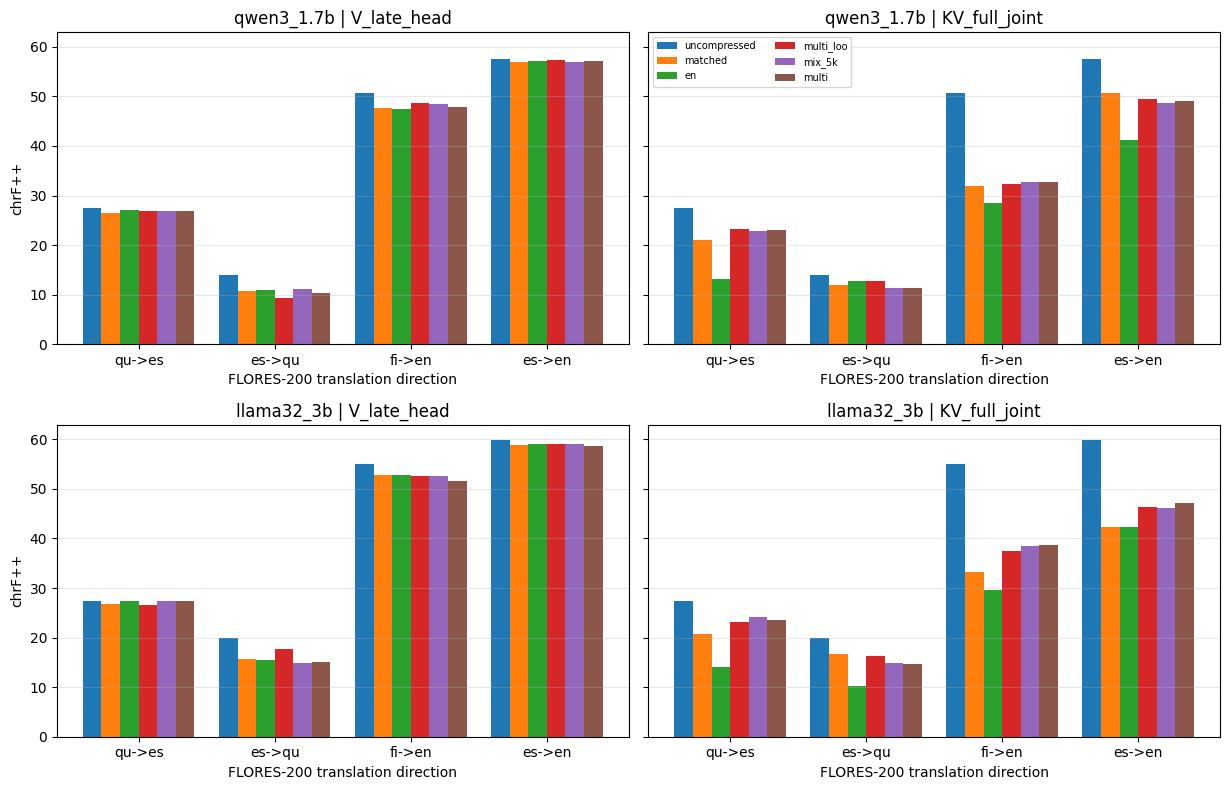
\includegraphics[width=\linewidth]{week7_fig2_mt_flores_downstream.png}
  \caption{FLORES-200 autoregressive machine translation chrF++ ($N=80$, 5-shot, real \texttt{use\_cache=True} KV-cache compression) across Qwen3-1.7B (top) and Llama-3.2-3B (bottom). While mild \texttt{V\_late\_head} is resilient (left), full-model $4\times$ \texttt{KV\_full\_joint} under English-only calibration collapses \texttt{qu$\rightarrow$es}, \texttt{es$\rightarrow$qu}, and \texttt{fi$\rightarrow$en}, and is restored by \texttt{mix\_5k} (right).}
  \label{fig:downstream}
\end{figure*}

\paragraph{Mild vs.\ Realistic Full-Model Compression.}
Under mild \texttt{V\_late\_head} compression, short discriminative classification and translation are largely robust (notable exception: Llama-3.2 SIB-200 Finnish drops $-6.37\text{ pp}$ $[-10.29, -2.94]$ under \texttt{en} calibration, restored to $79.9\%$ by \texttt{mix\_5k}). Under realistic $4\times$ full-model decoding (\texttt{KV\_full\_joint}), however, English calibration causes severe downstream failure across both models.

\paragraph{Qualitative Failure Mode: Language-Collapse into English.}
Inspection of generated \texttt{qu}$\rightarrow$\texttt{es} translations under \texttt{KV\_full\_joint} reveals why chrF++ plunges by $-13.5$ to $-14.3$ points: \textbf{English-calibrated projectors pull the decoder out of Spanish and literally collapse output into repetitive English} (Table~\ref{tab:qualitative}). Replacing the English basis with \texttt{mix\_5k} restores Spanish generation and named entities, gaining $+9.6$ chrF++ on Qwen3 ($13.26\rightarrow 22.85$) and $+10.1$ chrF++ on Llama-3.2 ($14.01\rightarrow 24.14$, recovering $88\%$ of uncompressed $27.47$).

\paragraph{Why \texttt{mix\_5k} Beats Even Monolingual \texttt{matched} Calibration on Bilingual Prompts.}
A surprising and practical finding emerges on bilingual downstream tasks: in both SIB-200 (English instructions/labels + Quechua input text) and MT (\texttt{qu}$\rightarrow$\texttt{es}, \texttt{fi}$\rightarrow$\texttt{en}), the KV cache holds \emph{two languages simultaneously}. Consequently, \emph{any} monolingual basis penalizes the other language in the prompt: on Llama-3.2 SIB-200 \texttt{qu}, both \texttt{en}-only ($35.3\%$) and \texttt{qu}-only \texttt{matched} ($33.3\%$) collapse, whereas \texttt{mix\_5k} jumps to $\mathbf{52.0\%}$ ($+18.63\text{ pp}$ over \texttt{matched}, $[+13.24, +24.51]$). Similarly, on Llama-3.2 \texttt{qu}$\rightarrow$\texttt{es} and \texttt{fi}$\rightarrow$\texttt{en}, \texttt{mix\_5k} outperforms \texttt{matched} by $+3.5$ and $+5.4$ chrF++.

\begin{table}[t]
\centering
\footnotesize
\begin{tabular}{p{1.65cm}p{5.55cm}}
\toprule
Condition & Generated \texttt{qu$\rightarrow$es} Output (FLORES \texttt{devtest} \#2) \\
\midrule
\textbf{Reference} & \textit{La investigaci{\'o}n todav{\'i}a se ubica en su etapa inicial, conforme indicara el Dr.\ Ehud Ur, docente en la carrera de medicina de la Universidad de Dalhousie\dots} \\
\midrule
\textbf{Qwen3 Uncomp.} & Dr.\ Ehud Ur, m{\'e}dico de la Universidad de Dalhosie, ha sido nombrado director de la Divisi{\'o}n Cl{\'i}nica de la Universidad de Nueva Escocia. \\
\textbf{Qwen3 \texttt{en}-cal.} & \textcolor{red!70!black}{\texttt{The pilot was the first to be identified in the world, and the first to be identified in the world\dots}} \\
\textbf{Qwen3 \texttt{mix\_5k}} & El Dr.\ Ehud Ur, el director de la escuela de medicina de la Universidad de Edinburgh, fue nombrado director\dots \\
\midrule
\textbf{Llama3.2 \texttt{en}-cal.} & \textcolor{red!70!black}{\texttt{Dr.\ Ehud Ur, yachachiq of the Dalhosie Suntur, was appointed as the new director of the clinic\dots He is a professor\dots}} \\
\textbf{Llama3.2 \texttt{mix\_5k}} & Dr.\ Ehud Ur, el director de la escuela de medicina, y el presidente de la divisi{\'o}n\dots \\
\bottomrule
\end{tabular}
\caption{Qualitative \texttt{qu}$\rightarrow$\texttt{es} translations under $4\times$ \texttt{KV\_full\_joint} compression. English-only calibration causes literal language-collapse into English in both models; \texttt{mix\_5k} preserves Spanish output.}
\label{tab:qualitative}
\end{table}

% ============================================================================
\section{Practical Recommendations}
Our results translate directly into four deployment guidelines for low-rank KV-cache compression in multilingual LLMs:
\begin{enumerate}
  \item \textbf{Always protect position~0 (\texttt{protect\_pos0=True}):} Exempting a single sink token prevents catastrophic \texttt{K} collapse in QK-Norm models ($-150$--$325\%$ PPL) and cuts \texttt{K} error up to $5.5\times$ in standard attention models, at negligible memory cost ($1/T$).
  \item \textbf{Use layer-wide \texttt{joint} KV projectors over per-head projectors:} At identical rank budget, \texttt{joint} reduces cross-lingual NLL loss by up to $76\%$ and adaptively reallocates rank across heads.
  \item \textbf{Project Keys after \texttt{k\_norm} when QK-Norm is present} and leave early sink-forming layers (layers 0--2) uncompressed when targeting $4\times$ full-model \texttt{K+V} compression.
  \item \textbf{Include $\sim$5k tokens per low-resource language ($w=0.05$--$0.10$) in the calibration mixture:} Even minimal Wikipedia slices eliminate $97$--$100\%$ of parallel perplexity bias, prevent language-collapse into English during decoding, and beat every monolingual basis on bilingual prompts.
\end{enumerate}

% ============================================================================
\section{Limitations}
First, all four languages studied use the Latin script; extending our evaluation to non-Latin low-resource scripts (e.g., Ethiopic, Myanmar, Devanagari) is an important next step to disentangle script shift from resource scarcity. Second, our experiments cover 1.7B--3B parameter models runnable on single-GPU consumer hardware; scaling to 7B--70B models may alter the exact rank threshold where \texttt{V} subspaces diverge. Third, we study unweighted uncentered Gram SVD projectors; evaluating query-weighted or Fisher-weighted projections (as in Palu) under our cross-lingual protocol remains future work. Finally, our evaluations use $512$--$1024$-token contexts; long-context retrieval ($8\text{k}$--$32\text{k}$) may amplify cumulative KV-cache drift.

% ============================================================================
\section{Conclusion}
English-only calibration in low-rank KV-cache compression is not language-neutral. Across both Qwen3-1.7B and Llama-3.2-3B, on held-out Wikipedia, strictly parallel FLORES-200, and downstream SIB-200 and autoregressive translation benchmarks, we show that cross-lingual calibration bias concentrates in Value states, escalates into forced language-collapse into English under $4\times$ full-model decoding, and coexists with a previously overlooked position-0 attention-sink failure amplified by QK-Norm. Fortunately, the remedy is remarkably lightweight: protecting a single sink token, sharing projections across heads, and mixing just $\sim$5k tokens of each low-resource language into the calibration Gram restores equitable multilingual inference.

% ============================================================================
\section*{Reproducibility Statement}
All eight self-contained Jupyter notebooks, 25 extracted figures, and complete quantitative tables are publicly archived at \url{https://github.com/Disentangle-Lab/kv-cache-low-resources} and permanently versioned on Zenodo (\texttt{doi:10.5281/zenodo.24619734}). Every experiment runs on a single 16\,GB T4 GPU using ungated open weights and public datasets.

\bibliographystyle{plainnat}
\bibliography{references}

\end{document}
